% Procedure for installation

\stepcounter{tableCounter} % Increment counter
\setcounter{rowCounter}{0} % Reset counter
\begin{tabularx}{\textwidth}{|>{\columncolor{tableColumnColor}}c|>{\columncolor{tableColumnColor}}c|>{\hsize=1.2\hsize}X|>{\hsize=.8\hsize}X|}
  \hline
  \rowcolor{tableHeaderColor}
  ID & Check & Description & Comments \\ \hline

  \procedureItem{Clean table and cover work-area with paper}{}
  
  \procedureItem{Make sure to wear gloves during the whole assembly/cleaning}{}
  
  \procedureItem{Define dirty and clean area (left, right)}{}
  
  \procedureItem{Lay out parts on area for dirty parts of clean table 
Parts: 
\begin{itemize}
  \item 1x Igniter Body
  \item 1x Sparkplug
  \item 1x Pressure sensor (NAT 8352)
  \item 3x $\frac{1}{4}$” Swagelok fitting ($\frac{1}{4}$” Swagelok tube connection to G $\frac{1}{4}$" male thread)
  \item 4x $\frac{1}{4}$” Copper gasket (unused/visibly not damaged)
  \item 2x $\frac{3}{8}$” Novapress Universal Holländer Dichtung
  \item 2x Hovadur Nut
  \item 1x Hovadur Hollow Screw
\end{itemize}

Tools:
\begin{itemize}
  \item 2x Adjustable wrench (alternatively SW 21/22)
  \item GTR table clamp
\end{itemize}
Material:
\begin{itemize}
  \item Acetone
  \item Isopropanol
  \item Distilled water
  \item Gloves
  \item Paper towel
  \item Teflon tape ($\frac{3}{8}$”)
\end{itemize}}{}
  
  \procedureItem{Inspect all parts for damage (especially copper gaskets)}{}
  
  \procedureItem{Clean parts as following: 
(Do not clean interior of valves and anything that contains plastic with acetone or other chemicals, only distilled water can be used. Putting a bit on a paper towel to clean threads is ok, as long as no rubber is near it.) 

Cleaning for Oxygen Service (CFOS of OSS all the lines, Igniter Oxygen line):
\begin{itemize}
  \item Check sealings compatibility
  \item Wear gloves (latex/nitril) during all operations
  \item Place parts on clean plastic foil
  \item Organize Disassembly/Assembly
  \item For small parts (e.g., fittings) perform ultrasonic bath cleaning
\end{itemize}

\textbf{Hydrogen} as Fuel:
\begin{itemize}
  \item Cleaning for Oxygen Service (CFOS of Purging lines, FSS all lines, Igniter Fuel lines):
  \item Check sealings compatibility
  \item Wear gloves (latex/nitril) during all operations
  \item Place parts on clean plastic foil
  \item Organize Disassembly/Assembly
  \item For small parts (e.g., fittings) perform ultrasonic bath cleaning
\end{itemize}}{}
  
  \procedureItem{Pictures to get the general orientation:
  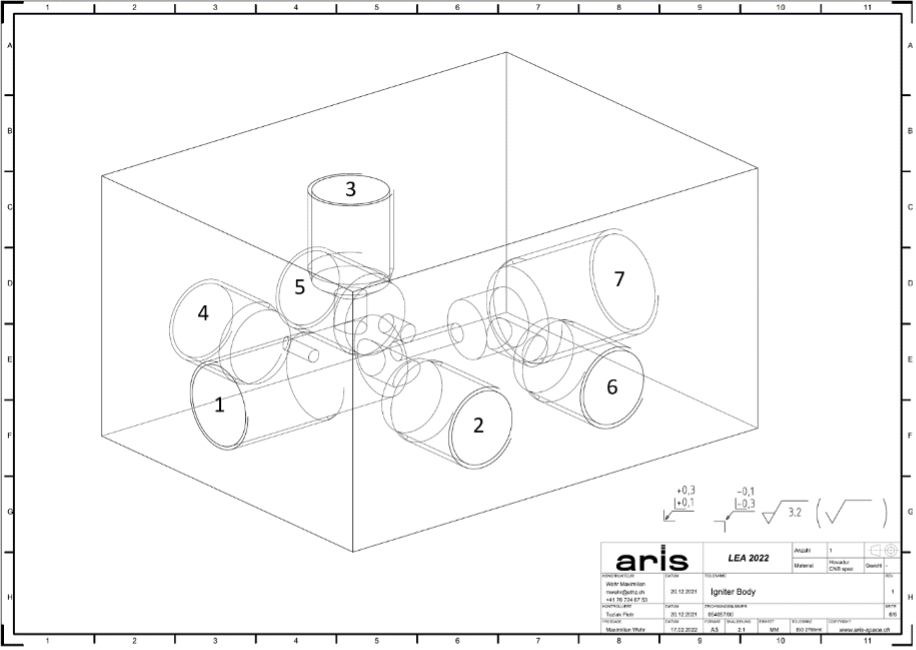
\includegraphics[width=\textwidth]{assets/technical_drawing.png}


1. Connection to sparkplug, 2. Fuel inlet, 3. Oxygen inlet, 4. Pressure sensor connection, 5. Thermocouple connection, 6. Fuel bypass, 7. Connection to engine}{}
  
  \procedureItem{Igniter assembled (without thermocouple)
  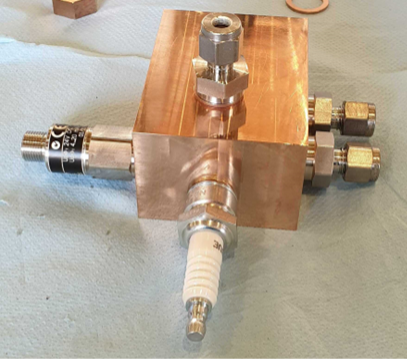
\includegraphics[width=\textwidth]{assets/full_assembly.png}}{}
  
  \procedureItem{Get Igniter Body and lay it on the side without connection such that the connection that is now on top is facing you (Oxygen) 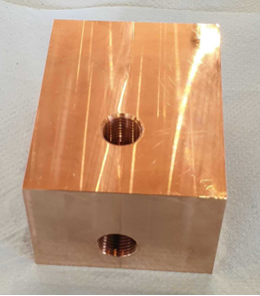
\includegraphics[width=\textwidth]{assets/step_1.png}}{}
  
  \procedureItem{Screw in topside $\frac{1}{4}$” Swagelok fitting (Oxygen) with an unused $\frac{1}{4}$” copper gasket hand tight}{}
  
  \procedureItem{Lay assembly on table edge, Oxygen inlet facing off the table, sparkplug facing left and Fuel inlets facing down 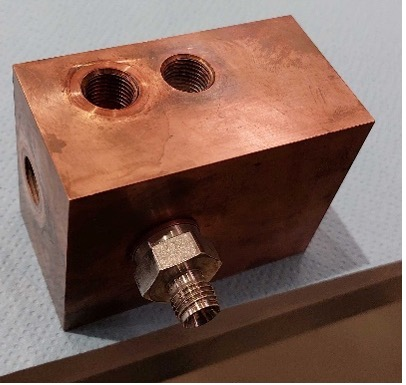
\includegraphics[width=\textwidth]{assets/step_2.jpg}}{}
  
  \procedureItem{Clamp igniter onto table with paper towels in-between, as to not damage the igniter. Place the clamp left of the to be tightened inlet, so it can better be tightened.}{}
  
  \procedureItem{Tighten the Fitting hard such that the metal gasket can properly seal}{}
  
  \procedureItem{Unclamp the igniter}{}
  
  \procedureItem{Lay igniter on side without connections again near the edge of the table to be clamped down}{}
  
  \procedureItem{Fuel Inlets need to face off the table  
(ATTENTION: all double inlets are $\frac{1}{4}$”) 
Sparkplug faces left
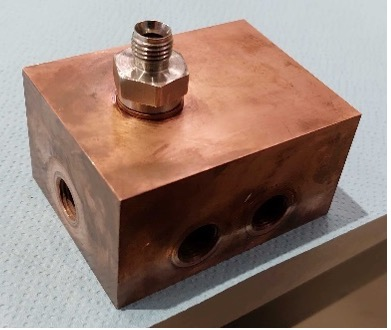
\includegraphics[width=\linewidth]{assets/step_3.jpg}
}{}
  
  \procedureItem{Clamp igniter onto table with paper towels in-between, as to not damage the igniter. Place the clamp left of the to be tightened inlet, so it can better be tightened.}{}
  
  \procedureItem{Screw in $\frac{1}{4}$” Swagelok fitting (Fuel) with an unused $\frac{1}{4}$” copper gasket hand tight}{}
  
  \procedureItem{Tighten the Fitting hard such that the metal gasket can properly seal}{}
  
  \procedureItem{Screw in $\frac{1}{4}$” Swagelok fitting (Bypass) with an unused $\frac{1}{4}$” copper gasket hand tight}{}
  
  \procedureItem{Tighten the Fitting hard such that the metal gasket can properly seal}{}
  
  \procedureItem{Unclamp the igniter}{}

  \procedureItem{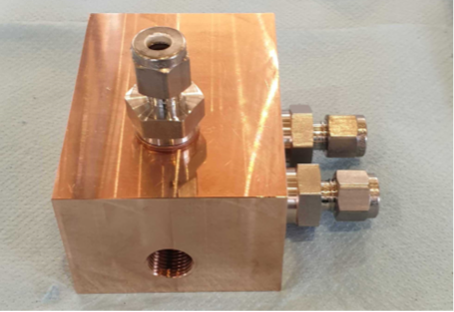
\includegraphics[width=\textwidth]{assets/step_4.png}}{}
  
  \procedureItem{Connect Sparkplug (has metal-sealing permanently connected) 
Don’t overtighten, the sealing is very compressible and doesn’t need tightening until it cannot be turned anymore 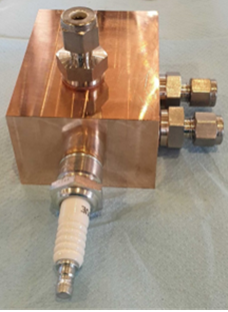
\includegraphics[width=\textwidth]{assets/step_5.png}}{}
  
  \procedureItem{Connect the Pressure sensor on the left side in the connection near to the sparkplug. Use a copper gasket here as well (see next step) (Thread-depth is not enough for the sensor to fit otherwise) (should have rubber seal permanently installed on the pressure sensor, if missing do not install and find replacement)}{}
  
  \procedureItem{Screw in Pressure sensor with unused $\frac{1}{4}$” copper gasket hand tight}{}
  
  \procedureItem{Lay igniter on side without connections, again near the edge of the table to be clamped down}{}
  
  \procedureItem{Clamp igniter onto table with paper towels in-between, as to not damage the igniter. Place the clamp left of the to be tightened inlet, so it can better be tightened.}{}
  
  \procedureItem{Tighten the Pressure sensor hard such that the metal gasket can properly seal}{}
  
  \procedureItem{Take Hovadur Hollow Screw}{}
  
  \procedureItem{Take Hovadur Nut}{}
  
  \procedureItem{Screw Nut on Hollow Screw until the nut is 1/2 up the thread}{}
  
  \procedureItem{Take one “$\frac{3}{8}$” Novapress Universal Holländer Dichtung” and put it on one side of the nut}{}
  
  \procedureItem{Screw the side with the gasket into the igniter}{}
  
  \procedureItem{Tighten the nut such that the gasket can properly seal}{}
  
  \procedureItem{Use the thermal paste and screw the thermocouple into the hole next to the pressure sensor and tighten}{}
  
  \procedureItem{Unclamp the igniter}{}
  
  \procedureItem{Keep second “$\frac{3}{8}$” Novapress Universal Holländer Dichtung” stored together with assembled igniter for further engine assembly}{}
  
\end{tabularx}
